%
% einleitung.tex -- Beispiel-File für die Einleitung
%
% (c) 2020 Prof Dr Andreas Müller, Hochschule Rapperswil
%
% !TEX root = ../../buch.tex
% !TEX encoding = UTF-8
%
\section{Brownische Bewegung\label{brown:section:teil0}}
\rhead{Brownische Bewegung}

Als der Schottische Botaniker Robert Brown im Jahr 1827 in sein Mikroskop schaut, beobachtet er kleine Partikel von Pflanzenpollen in einer Flüssigkeit. Er bemerkt, dass sich die Teilchen scheinbar zufällig bewegen, obwohl scheinbar keine Kräfte auf die Teilchen einwirken. Eine abschliessende Erklärung hatte Robert Brown zu diesem Zeitpunkt für das Verhalten noch nicht.\\

%ToDo: Mehr ins Detail?


Es dauerte fast ein Jahrhundert, bis Albert Einstein diese Beobachtung auf ein solides theoretisches Fundament stellte und nutzbar machte. Er schloss darauf, dass dir unregelmäßige Bewegung auf Kollisionen mit umgebenden Molekülen zurückzuführen ist, welche ständig in Bewegung sind. Albert Einstein entwickelte eine Mathematische Theorie, mit welcher die beobachtete Bewegung mit stochastischen Zusammenstößen von Molekülen erklärt werden kann. So konnte er auch einen Zusammenhang zwischen Messungen der Bewegung, der Bolzmankonstante und der  Avogadrozahl herstellen.\footnote{Die Avogadrozahl ($N_\mathrm{A}$) ist die Anzahl der Teilchen (Atome oder Moleküle) in einem Mol einer Substanz. Die Boltzmannkonstante ($k$) ist eine physikalische Konstante, die den Zusammenhang zwischen der thermischen Energie und der Temperatur eines Systems herstellt. Beide Konstanten sind miteinander verbunden durch die Gleichung $k = \frac{R}{N_\mathrm{A}}$, wobei $R$ die allgemeine Gaskonstante ist.}\\


Dies hatte auch Auswirkungen auf das Verständnis von Materie, da es empirische Belege für die Existenz für Atomen und Moleküle liefert. Die Atomhypothese besagt, dass Materie aus diskreten unteilbaren Einheiten besteht. Diese diskreten Einheiten entsprechen einzelnen Atomen oder ganzen Molekülen. 

Man muss dazu sagen, dass es schon zuvor Indizien für deren Existenz gab, doch es fehlte am entscheidenden experimentellen Beweis.\\


Die Einstein-Smoluchowski-Gleichung ist eine zentrale Gleichung seiner Arbeit beschreibt die mittlere quadratische Verschiebung (MSD: "Mean square displacement"),

\begin{equation}
	\mathrm{MSD} = 2nDt
\end{equation}

in Beziehung zur Diffusionskonstanten $ D $ , der Anzahl Raumdimensionen $ n $ und der Zeit $ t $.\\


Die Avogadrozahl $ \mathrm{A} $ kann indirekt über die Stokes-Einstein-Gleichung, anhand von Messungen berechnet werden.

\begin{equation}
	D = \frac{kT}{6\pi\eta r}
\end{equation}

$ r $ beschreibt dabei den Radius des suspendierten Teilchens, $ k $ die Boltzmann-Konstante, $ T $ die Temperatur und $ \eta $ die Viskosität des umgebenden Mediums.\\


Die Avogadrozahl $ \mathrm{A} $ kann anhand dieser beiden Gleichungen über die Boltzmannkonstante $ k $ berechnet werden. Diese ist definiert als $ k = R/\mathrm{A} $. $ R $ ist dabei die allgemeine Gaskonstante, welche gemäss der idealen Gasgleichung $ PV = nRT $ zu bestimmen ist. Es ergibt sich folgender Zusammenhang:

\begin{equation}
	\mathrm{A} = \frac{R T}{D (6 \pi \eta r)}
\end{equation}


So ermöglichen die beiden Gleichungen einen experimentellen Ansatz zur Bestimmung der Avogadro-Konstante und ferner zur quantitativen Analyse der Brownischen Bewegung.




\subsection{Simulation mittels der Euler-Maruyama-Methode
\label{brown:section:teil0}}

Die Brownische Bewegung kann relativ einfach simuliert werden mittels der Eueler-Maruyama-Methode.\\


Die Euler-Maruyama-Methode ist eine numerische Methode zur Simulation von stochastischen Differentialgleichungen (SDE). SDEs sind Differenzialgleichungen, welche den Einfluss von zufälligen Prozessen, wie zum Beispiel Rauschen, auf ein dynamisches System berücksichtigen können. Sie bestehen aus einem deterministischen Anteil, der die zugrundeliegende Dynamik beschreibt, und einem stochastischen Anteil, der einen zufälligen Einfluss in Betracht zieht. Die Methode basiert auf der bekannten Euler-Methode zur Lösung von gewöhnlichen Differentialgleichungen (ODEs). Die Idee ist, die SDE in diskrete Zeitschritte zu zerlegen und den deterministischen und stochastischen Anteil separat zu behandeln. Die Methode hat zwar gewisse Einschränkungen hinsichtlich ihrer Genauigkeit und Stabilität, ist aber dennoch mitunter auf Grund ihrer Einfachheit weit verbreitet.\\


Gegeben sei eine SDE der folgenden Form:

\begin{equation}
	\mathrm{d}X(t) = a(X(t), t) \mathrm{d}t + b(X(t), t) \mathrm{d}W(t),
\end{equation}

wobei $X(t)$ die gesuchte Funktion, $a(X(t), t)$ der deterministische Anteil, $b(X(t), t)$ der stochastische Anteil und $W(t)$ ein Wiener-Prozess ist, der das Rauschen repräsentiert. Die Methode beginnt mit einer Anfangsbedingung $X(0) = X_0$.\\


Um die SDE mit der Euler-Maruyama-Methode zu simulieren, geht man wie folgt vor:

\begin{enumerate}
	\item Man wählt eine Schrittweite $\Delta t > 0$ und teilt das Zeitintervall $[0, T]$ in $N$ gleich große Teilintervalle der Länge $\Delta t$: $t_0 = 0, t_1 = \Delta t, \dots, t_i = i\Delta t, \dots, t_N = T$.
	\item Für jeden Zeitschritt $i$ von $0$ bis $N-1$ werden die Werte der Funktion $X(t)$ an den diskreten Zeitpunkten $t_i$ berechnet,
	\begin{equation}
		X(t_{i+1}) = X(t_i) + a(X(t_i), t_i) \Delta t + b(X(t_i), t_i) \sqrt{\Delta t} \cdot Z_i,
	\end{equation}
	wobei $Z_i$ unabhängige standardnormalverteilte Zufallsvariablen sind.
	\item Diese Berechnungen führt man iterativ für alle Zeitschritte durch.
\end{enumerate}

\begin{equation}
	X_{n+1} = X_n + f(X_n,t_n) \Delta t + g(X_n,t_n) \Delta W_n
\end{equation}

Diese Funktion $ f(X_n,t_n) $ beschreibt dabei den deterministischen Teil der SDE, im Kontext der Brown'schen Bewegung kann man es auch "drift nennen", welcher nicht nur von zufälligen Einflüssen bestimmt ist. Dies ist auch der Teil, der durch eine harmonische Analyse untersucht werden kann. Das Rauschen ("white noise"), welches hier mit $ g(X_n,t_n) $ beschrieben ist, enthält keine Information und kann somit nicht analysiert werden. $ \Delta W $ beschreibt die Geschwindigkeit, mit welcher der stochastische Prozess ablaufen soll und $ W_n $  beschreibt den Wiener Prozess oder die Brownische Bewegung als Ganzes.\\


\begin{figure}[h!]
	\centering
	\begin{minipage}{0.45\textwidth}
		\centering
		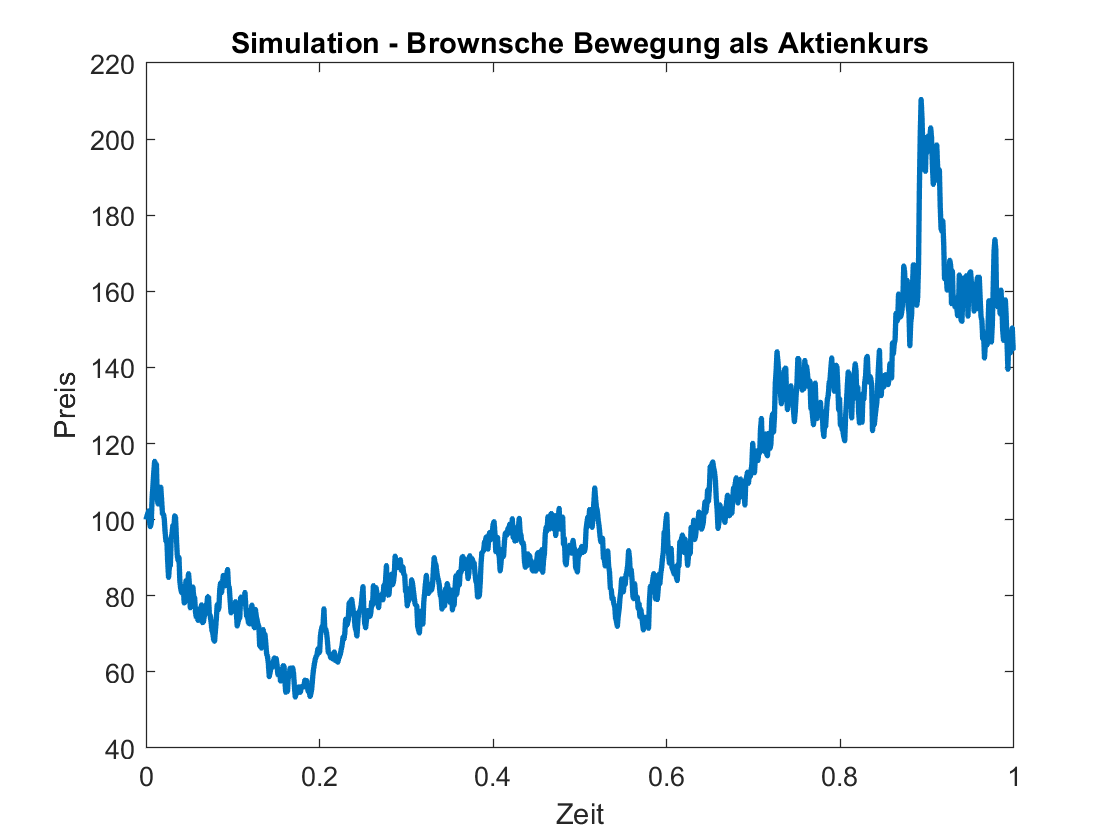
\includegraphics[width=\linewidth]{papers/brown/images/Aktienkurs-als-Brownische-Bewegung_2.png}
		\caption{Euler-Maruyama-Methode in 1D}
	\end{minipage}
	\hspace{0.05\linewidth}
	\begin{minipage}{0.45\textwidth}
		\centering
		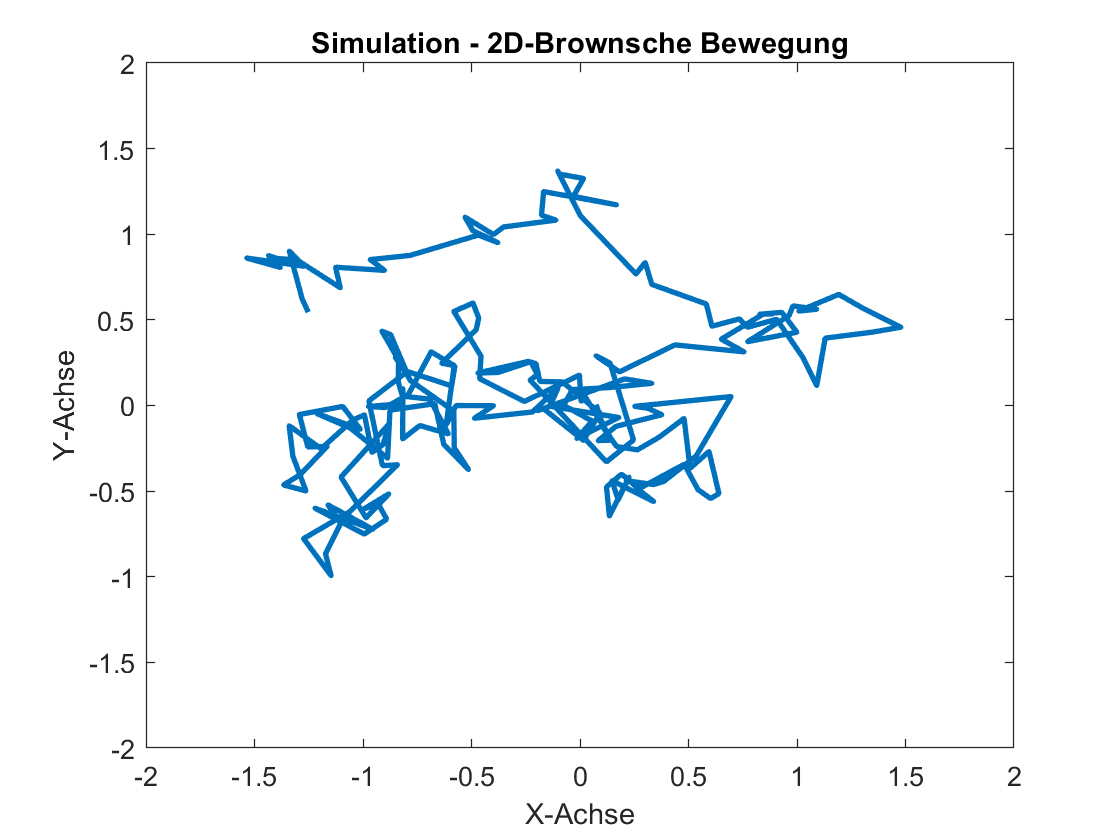
\includegraphics[width=\linewidth]{papers/brown/images/Brownische-Bewegung-Simuliert_2.png}
		\caption{Simulation einer Brownischen Bewegung}
	\end{minipage}
\end{figure}

In der Abbildung ... ist wurde diese Simulations-Methode in einer Dimension angewandt. Man kann vielleicht schon erahnen, dass die zugrundeliegende Mathematik auf Börsenkurse anwendbar sein könnte. Führt man die Simulation für zwei Achsen durch und verbindet die einzelnen Simulationsschritte mit Linien, ergibt sich das Bild einer typischen Brownischen Bewegung.


%\begin{figure}
%	\centering
%	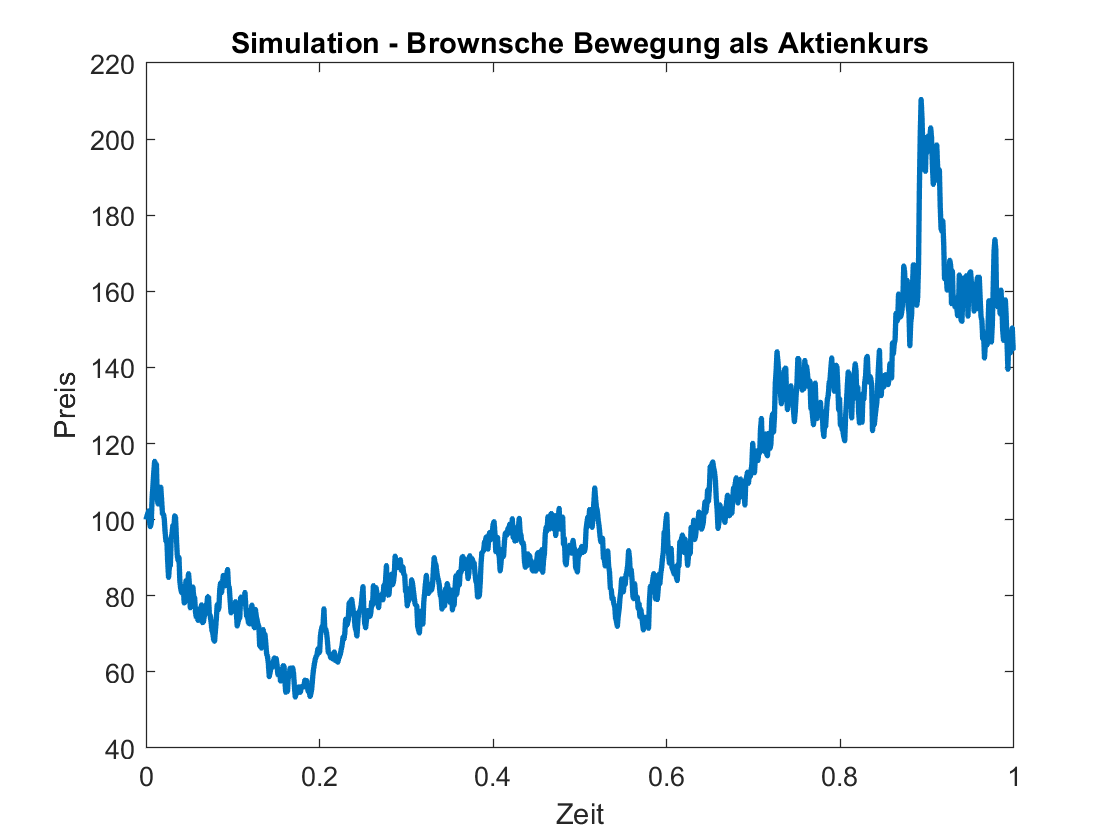
\includegraphics[width=0.7\linewidth]{papers/brown/images/Aktienkurs-als-Brownische-Bewegung_2.png}
%	\caption{Simulation mittels der Eueler-Maruyama-Methode eines Aktienkurses}
%\end{figure}
%
%\begin{figure}
%	\centering
%	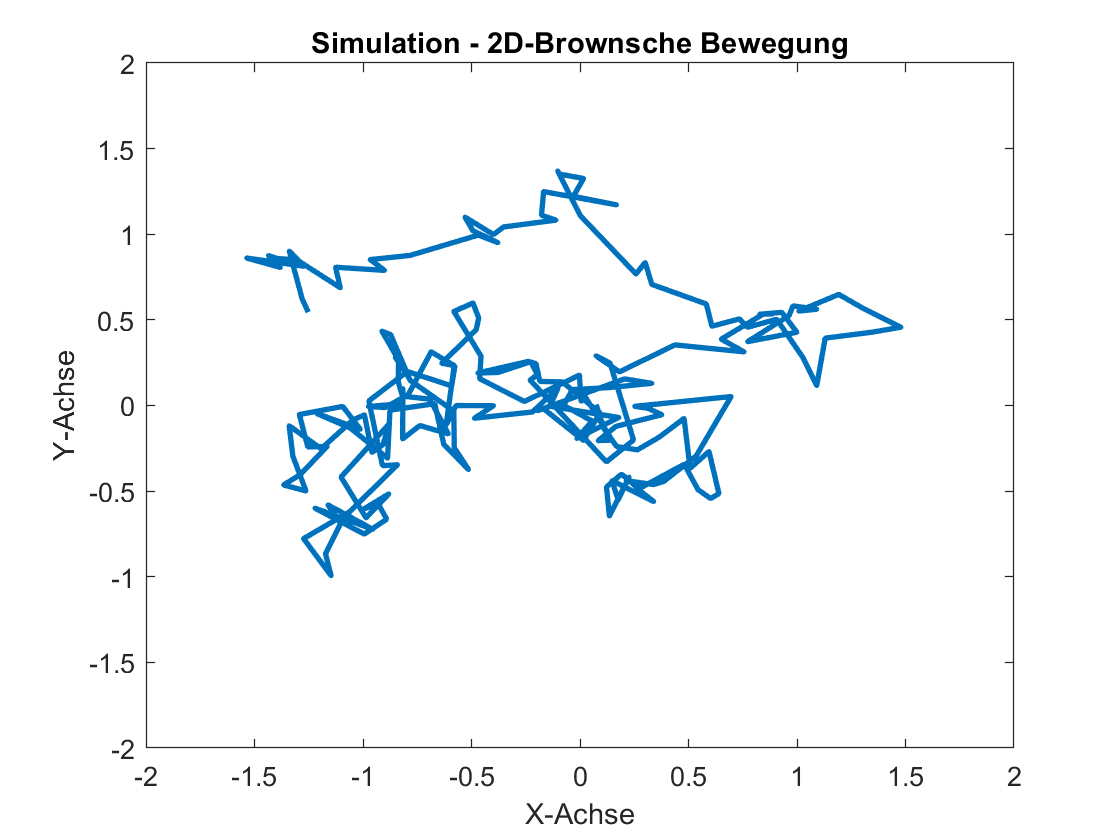
\includegraphics[width=0.7\linewidth]{papers/brown/images/Brownische-Bewegung-Simuliert_2.png}
%	\caption{Simulation mittels der Eueler-Maruyama-Methode der Brown'schen Bewegung eines Teilchens}
%\end{figure}